\documentclass[12pt,a4paper]{article}

\usepackage[T2A]{fontenc}
\usepackage[utf8]{inputenc}
\usepackage[russian]{babel}
\usepackage{amsmath,amssymb}
\usepackage{graphicx}
\usepackage{booktabs}
\usepackage{geometry}
\geometry{margin=2.4cm}
\usepackage{tikz}
\usetikzlibrary{arrows.meta,positioning,shapes.geometric}
\usepackage{float}
\usepackage{caption}
\captionsetup{labelsep=endash}
\usepackage{hyperref}
\hypersetup{colorlinks=true,linkcolor=black,urlcolor=blue}

\title{Лабораторная работа №\,2\\ \large Генетический алгоритм для дискретной задачи с ограничениями (распределение заявок между исполнителями)}
\author{Панов Артемий, Б24-527}
\date{2026 г.}

\begin{document}
\maketitle

\section{Постановка задачи и индивидуальный вариант}

Требуется решить задачу распределения заявок между исполнителями с различной
производительностью при ограничении ёмкости каждого исполнителя
генетическим алгоритмом с целочисленным кодированием.

Индивидуальные параметры: $N = 18$, $Q = 2$ (группа 527), $Y = 26$. Номер
варианта:
\[
V = 1 + \big((17N + 7Q + Y) \bmod 20\big) = 1 + (346 \bmod 20) = 7.
\]

\textbf{Вариант 7 --- распределение ограниченного числа заявок между
исполнителями с различной производительностью}; основное представление ---
целочисленный вектор.

\section{Формальная модель и данные}

Есть $N = 30$ заявок с трудоёмкостями $w_i > 0$ и $M = 6$ исполнителей с
производительностью $p_j$ (объём в час) и ёмкостью $c_j$ (максимум заявок).
Назначение $x_i \in \{1, \dots, M\}$ для каждой заявки; время обработки
заявки $i$ исполнителем $j$ равно $t_{ij} = w_i / p_j$. Цель --- минимизировать
максимальное время завершения (makespan):
\[
\min_x \; T(x) = \max_{j} \sum_{i:\,x_i=j} \frac{w_i}{p_j}
\qquad
\text{s.t.}\quad \bigl|\{i : x_i = j\}\bigr| \le c_j \;\; \forall j.
\]

Экземпляр --- синтетический, генерируется с фиксированным зерном
$\text{seed} = 746$: трудоёмкости $w_i \sim \mathrm{U}(1, 10)$,
производительности $p = (0{,}5;\,0{,}7;\,1{,}0;\,1{,}3;\,1{,}6;\,2{,}0)$,
ёмкости $c = (5;\,6;\,7;\,6;\,5;\,6)$, $\sum c_j = 35 \ge 30$ --- допустимые
решения существуют. Минимальные масштабы по ТЗ выполнены: 30 заявок
$\ge 20$, 6 исполнителей $\ge 5$.

\section{Представление особи}

Особь --- целочисленный вектор $x = (x_1, \dots, x_{30})$,
$x_i \in \{0, \dots, 5\}$: элемент $i$ --- исполнитель заявки $i$. Такое
кодирование прямо отражает структуру решения (процедура декодирования
тривиальна), генетический материал --- это решения по каждой заявке, которые
рекомбинируются осмысленно.

\section{Генетический алгоритм}

Схема работы --- на рис.~\ref{fig:ga}, параметры --- в
таблице~\ref{tab:params}.

\begin{figure}[H]
\centering
\begin{tikzpicture}[
  node distance=0.45cm,
  box/.style={draw, rounded corners=2pt, align=center, minimum width=7.2cm,
              minimum height=0.85cm, font=\small},
  dec/.style={draw, diamond, aspect=2.6, align=center, font=\small, inner sep=1pt},
  arr/.style={-{Stealth[length=2.5mm]}, thick}]
\node[box] (init) {инициализация: 80 особей, равномерные назначения};
\node[box, below=of init] (eval) {оценка: makespan (+возможный штраф), допустимость};
\node[dec, below=of eval, yshift=-0.1cm] (stop) {бюджет $10^4$ исчерпан?};
\node[box, below=of stop, yshift=-0.3cm] (elite) {элитизм: 2 лучшие особи --- в потомство};
\node[box, below=of elite] (sel) {турнирная селекция родителей ($k = 3$)};
\node[box, below=of sel] (cross) {равномерный / одноточечный кроссовер ($p_c = 0{,}9$)};
\node[box, below=of cross] (mut) {мутация: переназначение гена ($p_m = 0{,}05$)};
\node[box, below=of mut] (repa) {ремонт (режим repair) либо нет (режим penalty)};
\node[box, right=2.2cm of stop] (end) {конец: лучший допустимый вектор};
\draw[arr] (init) -- (eval);
\draw[arr] (eval) -- (stop);
\draw[arr] (stop) -- node[left, font=\small]{нет} (elite);
\draw[arr] (elite) -- (sel);
\draw[arr] (sel) -- (cross);
\draw[arr] (cross) -- (mut);
\draw[arr] (mut) -- (repa);
\draw[arr] (repa.west) -| ++(-1.4,0) |- (eval.west);
\draw[arr] (stop) -- node[above, font=\small]{да} (end);
\end{tikzpicture}
\caption{Блок-схема генетического алгоритма}
\label{fig:ga}
\end{figure}

\begin{table}[H]
\centering
\small
\caption{Параметры алгоритма}
\label{tab:params}
\begin{tabular}{ll}
\toprule
Параметр & Значение \\
\midrule
Размер популяции & 80 ($\ge 30$ по заданию) \\
Селекция & турнирная, $k = 3$ \\
Рекомбинация & равномерный либо одноточечный кроссовер, $p_c = 0{,}9$ \\
Мутация & переназначение гена случайному исполнителю, $p_m = 0{,}05$ на ген \\
Обработка границ & ремонт либо штраф $W \cdot \sum_j \max(0, n_j - c_j)$, $W = 50$ \\
Сохранение лучшего & элитизм, 2 особи \\
Критерий остановки & бюджет $10\,000$ вычислений $f$ (инициализация включительно) \\
Серия & 30 независимых запусков, $\text{seed} = 8000 + 19i$ \\
\bottomrule
\end{tabular}
\end{table}

\textbf{Штраф.} $\text{fitness} = \max_j T_j + W \sum_j \max(0, n_j - c_j)$,
$W = 50$: за нарушение ёмкости добавляется большая константа.

\textbf{Ремонт.} Пока есть перегруженный исполнитель, переносится заявка от
него к свободному исполнителю, выбираемая по минимуму добавляемого времени
$w_i / p_k$ (жадный ремонт).

\section{Обоснование выбора операторов}

Структура задачи: назначения --- множество заявок с естественным
целочисленным кодением. Отсюда:
\begin{itemize}
\item \textbf{турнирная селекция} ($k = 3$) --- умеренное давление, не
  требующее масштабирования fitness (значения makespan порядка 25--50,
  но в ранних поколениях штрафные результаты разбегаются на сотни);
\item \textbf{равномерный и одноточечный кроссоверы} --- целочисленный
  вектор имеет смысловые элементы по заявкам; сравниваются два
  содержательно разных механизма обмена ответами по заявкам;
\item \textbf{мутация по гену} --- переназначение одной заявки случайному
  исполнителю, стандартная мелкая варьирующая операция для векторов
  назначений;
\item \textbf{рэмонт/штраф} --- два контрастных способа вернуть решения в
  допустимое множество, сравнение неформально отвечает на вопрос, какой
  работает лучше.
\end{itemize}

\section{Примеры допустимых и недопустимых решений}

\begin{table}[H]
\centering
\small
\caption{Проверка допустимости на четырёх решениях}
\label{tab:examples}
\begin{tabular}{clcl}
\toprule
№ & счёт по исполнителям & makespan & вердикт \\
\midrule
1 & (5, 6, 7, 6, 5, 1) & 54{,}842 & допустимо \\
2 & (5, 5, 5, 5, 5, 5) & 66{,}730 & допустимо \\
3 & (30, 0, 0, 0, 0, 0) & 377{,}898 & недопустимо (нарушение 25) \\
4 & (0, 0, 0, 0, 0, 30) & 94{,}475 & недопустимо (нарушение 24) \\
\bottomrule
\end{tabular}
\end{table}

\section{Методология эксперимента}

Три эксперимента, каждый --- по 30 независимых запусков
($\text{seed} = 8000 + 19i$) при фиксированном бюджете $10\,000$
вычислений:
\begin{enumerate}
\item \textbf{подход к ограничению}: штраф против ремонта
  (равномерный кроссовер у обоих);
\item \textbf{пара операторов}: равномерный против одноточечного кроссовера
  (в режиме ремонта --- победителя первого эксперимента);
\item \textbf{базовые линии}: лучшая конфигурация ГА против жадной
  эвристики LPT (заявки по убыванию $w_i$ назначаются допустимому
  исполнителю с наименьшей текущей длительностью) и случайного
  допустимого поиска (равномерные назначения с ремонтом, бюджет тот же).
\end{enumerate}

Метрики серии: лучшее, среднее, медиана, стандартное отклонение, худшее
значение; средние кривые сходимости с коридором мин--макс.

\section{Результаты: штраф против ремонта}

\begin{table}[H]
\centering
\small
\caption{Итоговый makespan по 30 запускам при двух подходах к ограничению}
\label{tab:constr}
\begin{tabular}{lccccc}
\toprule
Подход & Лучшее & Среднее & Медиана & Стд & Худшее \\
\midrule
штраф & 27{,}08 & 28{,}90 & 28{,}68 & 1{,}16 & 31{,}06 \\
ремонт & $\mathbf{26{,}80}$ & $\mathbf{27{,}17}$ & 27{,}18 & 0{,}20 & 27{,}48 \\
\bottomrule
\end{tabular}
\end{table}

\begin{figure}[H]
\centering
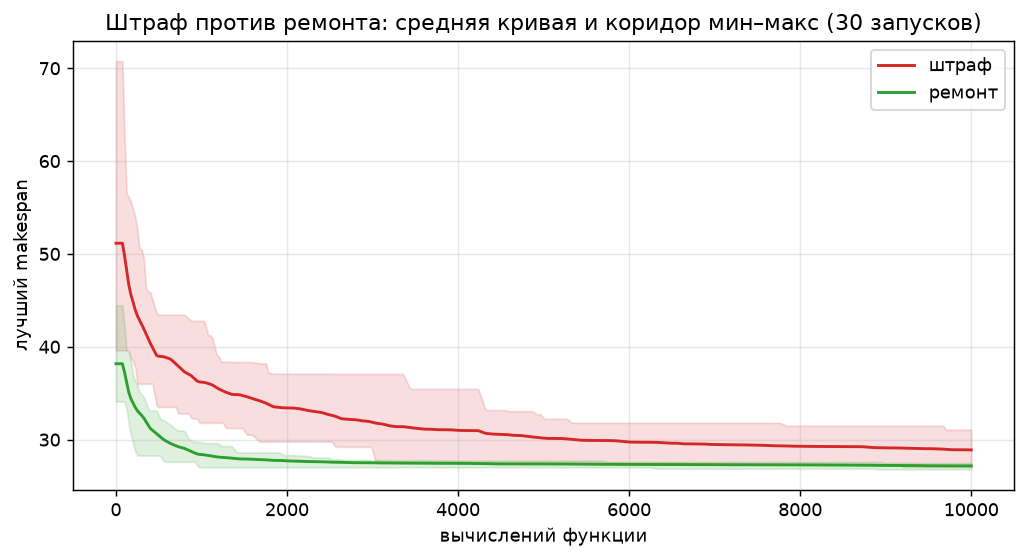
\includegraphics[width=0.86\textwidth]{figures/convergence_constraints.png}
\caption{Сходимость при двух подходах к ограничению}
\label{fig:constr}
\end{figure}

Ремонт устойчиво точнее штрафа (среднее 27{,}17 против 28{,}90,
таблица~\ref{tab:constr}, рис.~\ref{fig:constr}). При штрафе часть
популяции постоянно живёт с нарушениями: выигрыш в makespan у сильных
исполнителей часто больше штрафа $W = 50$, поэтому отбор ведёт в зону
нарушений (рис.~\ref{fig:feas}). Ремонт возвращает всех в допустимое
множество, отбор идёт по чистому makespan.

\begin{figure}[H]
\centering
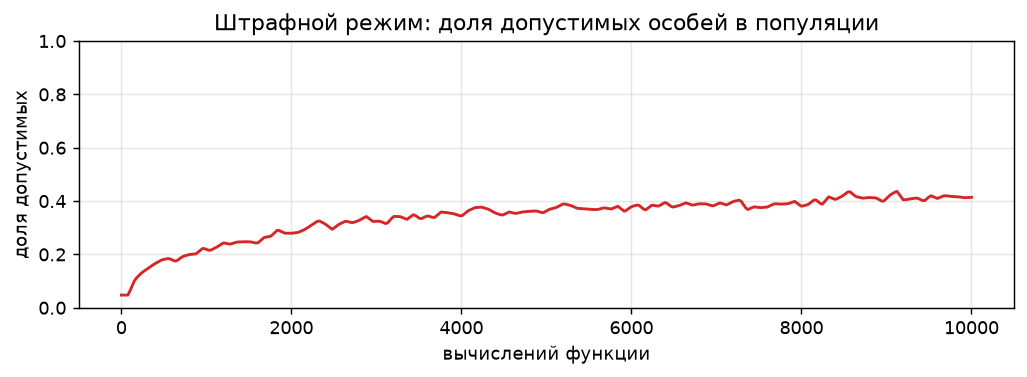
\includegraphics[width=0.86\textwidth]{figures/feasibility_penalty.png}
\caption{Штрафной режим: доля допустимых особей в популяции по поколениям}
\label{fig:feas}
\end{figure}

\section{Результаты: сравнение кроссоверов}

\begin{table}[H]
\centering
\small
\caption{Равномерный против одноточечного кроссовера (ремонт, 30 запусков)}
\label{tab:cross}
\begin{tabular}{lccccc}
\toprule
Кроссовер & Лучшее & Среднее & Медиана & Стд & Худшее \\
\midrule
равномерный & 26{,}80 & 27{,}17 & 27{,}18 & 0{,}20 & 27{,}48 \\
одноточечный & $\mathbf{26{,}72}$ & $\mathbf{27{,}00}$ & $\mathbf{27{,}00}$ & 0{,}17 & 27{,}41 \\
\bottomrule
\end{tabular}
\end{table}

\begin{figure}[H]
\centering
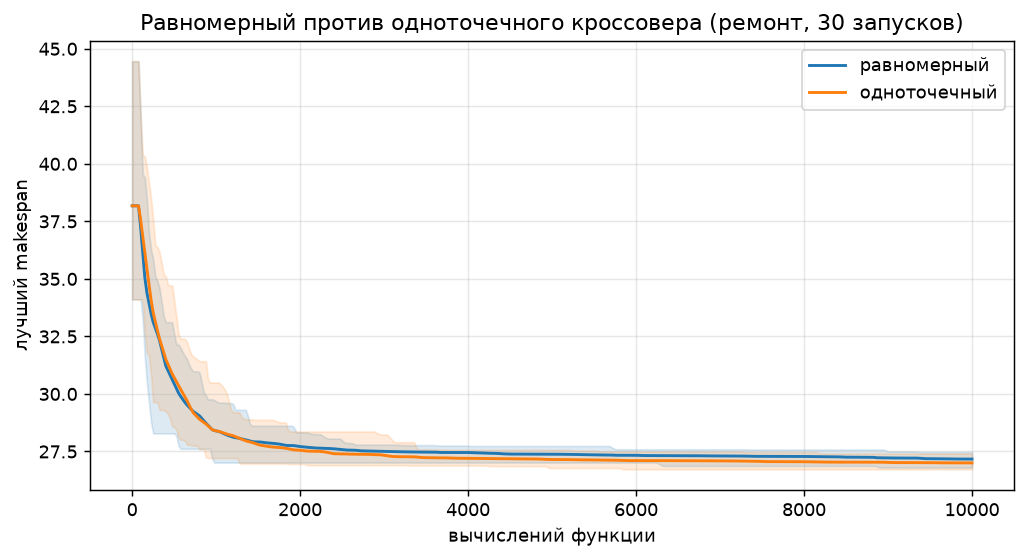
\includegraphics[width=0.86\textwidth]{figures/convergence_crossover.png}
\caption{Сходимость при двух операторах рекомбинации (режим ремонта)}
\label{fig:cross}
\end{figure}

Одноточечный кроссовер немного лучше равномерного --- разрыв
$27{,}00 \leftrightarrow 27{,}17$ (таблица~\ref{tab:cross},
рис.~\ref{fig:cross}) меньше стандартного отклонения, но стабилен по
среднему на 30 запусках. Равномерный разбивает слишком мелко; одноточечный
сохраняет пригодные участки ответов.

\section{Результаты: сравнение с базовыми линиями}

\begin{table}[H]
\centering
\small
\caption{ГА (одноточечный + ремонт) против жадной эвристики и случайного
допустимого поиска}
\label{tab:baselines}
\begin{tabular}{lc}
\toprule
Метод & makespan (среднее) \\
\midrule
ГА (одноточечный + ремонт), 30 запусков & $\mathbf{27{,}00}$ \\
случайный допустимый поиск (бюджет $10^4$), 30 запусков & 30{,}48 \\
жадная эвристика LPT & 33{,}69 \\
\bottomrule
\end{tabular}
\end{table}

\begin{figure}[H]
\centering
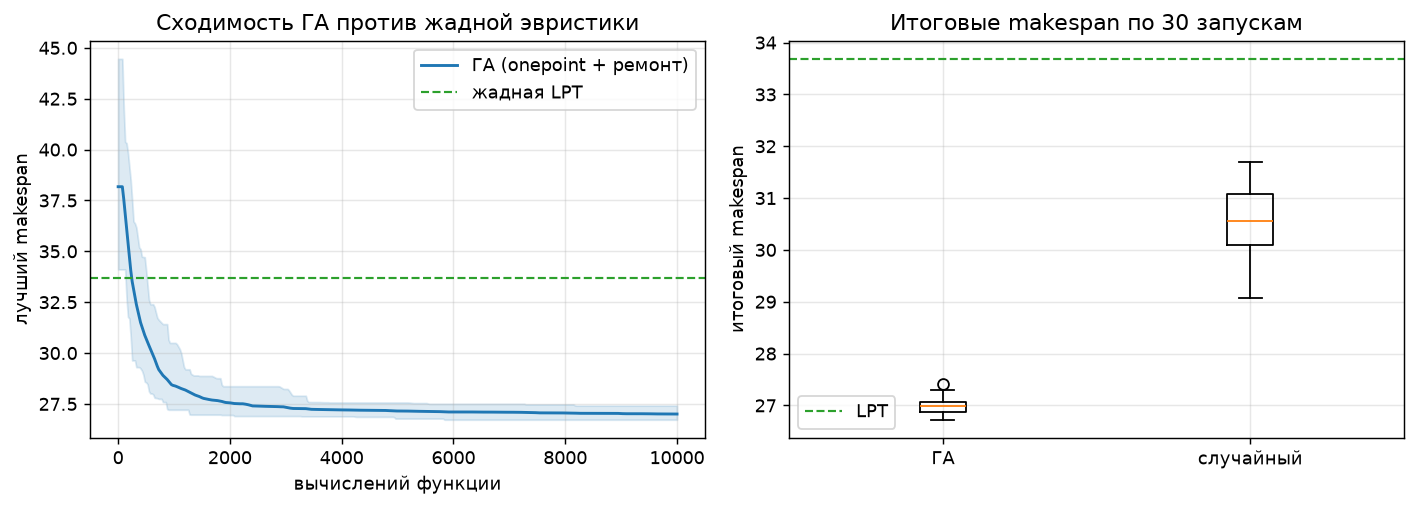
\includegraphics[width=0.98\textwidth]{figures/ga_vs_baselines.png}
\caption{Сходимость ГА против жадной эвристики (слева) и итоговые makespan
серий (справа)}
\label{fig:baselines}
\end{figure}

ГА устойчиво лучше обеих базовых линий (таблица~\ref{tab:baselines},
рис.~\ref{fig:baselines}): разрыв с жадной LPT --- около
$\frac{33{,}69 - 27{,}00}{33{,}69} \approx 20\%$, а случайный допустимый
поиск без селекции и рекомбинации стабилизирует только плотность бюджета
--- поэтому и проигрывает (лучшее значение $29{,}06$).

\textbf{Лучшее решение серии.} $x^*$ с makespan $26{,}724$; допустимость
по каждому исполнителю соблюдена (таблица~\ref{tab:best}).

\begin{table}[H]
\centering
\small
\caption{Лучшее решение по исполнителям (30 запусков ГА, best)}
\label{tab:best}
\begin{tabular}{cccccc}
\toprule
Исполнитель & Производительность & Ёмкость & Назначено & Длительность (ч) \\
\midrule
0 & 0{,}5 & 5 & 3 & 26{,}684 \\
1 & 0{,}7 & 6 & 4 & 26{,}441 \\
2 & 1{,}0 & 7 & 6 & 26{,}507 \\
3 & 1{,}3 & 6 & 6 & 26{,}675 \\
4 & 1{,}6 & 5 & 5 & 26{,}541 \\
5 & 2{,}0 & 6 & 6 & 26{,}724 \\
\bottomrule
\end{tabular}
\end{table}

\section{Оценка результата и выводы}

Полученный результат --- \textbf{хороший} для поставленной задачи: все
запуски в режиме ремонта дают допустимые решения по построению; лучшая
конфигурация (одноточечный кроссовер + ремонт) во всех 30 запусках находит
makespan $\le 27{,}41$, что лучше жадной эвристики на $\sim 20\%$ и
случайного допустимого поиска на $\sim 12\%$ --- это свойство алгоритма,
а не единичный удачный запуск.

Выводы:
\begin{enumerate}
\item ремонт устойчиво точнее штрафа (27{,}17 против 28{,}90) --- для
  ограничения ёмкости явное восстановление допустимости выигрывает у
  оценивания штрафом;
\item одноточечный кроссовер немного точнее равномерного в этой задаче
  (27{,}00 против 27{,}17), разница стабильна при фиксации всех прочих
  параметров;
\item ГА устойчиво улучшает жадную эвристику LPT (33{,}69 $\to$ 27{,}00)
  и случайный допустимый поиск (30{,}48 $\to$ 27{,}00);
\item лучшее makespan значение серии --- $26{,}72$ при полной допустимости.
\end{enumerate}

\section*{Состав материалов}

\begin{itemize}
\item \texttt{lab2.ipynb} --- ноутбук с полным кодом и всеми экспериментами;
\item \texttt{report.tex}, \texttt{report.pdf} --- настоящий отчёт;
\item \texttt{figures/convergence\_constraints.png} --- штраф против ремонта;
\item \texttt{figures/feasibility\_penalty.png} --- доля допустимых при штрафе;
\item \texttt{figures/convergence\_crossover.png} --- сравнение кроссоверов;
\item \texttt{figures/ga\_vs\_baselines.png} --- ГА против базовых линий;
\item \texttt{results/runs\_constraints.csv} --- запуски эксперимента 1;
\item \texttt{results/runs\_crossover.csv} --- запуски эксперимента 2;
\item \texttt{results/runs\_baselines.csv} --- запуски случайного поиска;
\item \texttt{results/summary\_constraints.csv},
  \texttt{results/summary\_crossover.csv} --- сводные статистики;
\item \texttt{results/best\_solution.csv} --- лучшее найденное назначение;
\item \texttt{README.md} --- инструкция по запуску и воспроизводимости.
\end{itemize}

\end{document}
